\documentclass[11pt]{article}

\usepackage[margin=1in]{geometry}
\usepackage{graphicx}
\usepackage{hyperref}
\usepackage{enumitem}
\usepackage{booktabs}

\title{TDC 2026 Final technical report\\[0.5em]
\large TTC Bus and Streetcar Delay Data Consolidation}
\author{The Delayticans}
\date{\today}

\hypersetup{
    colorlinks=true,
    linkcolor=blue,
    urlcolor=blue,
}

\begin{document}

\maketitle

\begin{abstract}
This report summarizes our work on the TDC 2026 project analyzing Toronto Transit Commission (TTC)
bus and streetcar delay data. We merged multi-year CSV datasets, built Python tooling to combine and
visualize the data, and produced charts that highlight rows with zero or null delay and gap values
across vehicle types and years.
\end{abstract}

\section{Introduction}

We are submitting our final report for the TDC 2026 project. Our team, The Delayticans, analyzed
publicly available TTC delay records for buses and streetcars. The goal was to consolidate fragmented
yearly datasets into unified files and explore data quality patterns that may affect downstream
analysis.

\section{Data Sources}

Raw CSV files are stored under \texttt{raw\_data\_sources/}, organized by vehicle type:

\begin{itemize}[noitemsep]
    \item \textbf{Buses} --- annual delay files from 2014 through 2024, plus a combined file for 2025 onward
    \item \textbf{Streetcars} --- annual delay files from 2014 through 2024, plus a combined file for 2025 onward
\end{itemize}

Each dataset includes delay-related fields such as \texttt{Min Delay} and \texttt{Min Gap}. Code
description files are provided alongside the raw data for reference.

\section{Methodology}

\subsection{CSV Merging}

We implemented \texttt{scripts/merge\_csv.py} to concatenate multiple CSV files in order. The script:

\begin{itemize}[noitemsep]
    \item writes a single header row from the first input file
    \item skips duplicate headers in subsequent files
    \item warns when headers differ between files
\end{itemize}

A companion runner, \texttt{scripts/merge\_csv\_run.py}, allows merging from the editor without using
the terminal. This workflow was used to combine monthly streetcar files into yearly datasets and to
prepare unified bus and streetcar files for analysis.

\subsection{Data Visualization}

We implemented \texttt{scripts/data\_visualiser.py} to generate charts from the merged datasets. For
each CSV file, the script counts rows where \texttt{Min Delay} or \texttt{Min Gap} is zero or null
and produces:

\begin{itemize}[noitemsep]
    \item a pie chart showing the proportion of affected rows versus all other rows
    \item a yearly bar chart summarizing the percentage of zero/null rows by vehicle type
\end{itemize}

Output figures are saved under \texttt{data\_visualisations/Buses/} and
\texttt{data\_visualisations/Streetcars/}.

\section{Completed Work}

We completed the following tasks for this submission:

\begin{enumerate}
    \item Merged CSV files for TTC bus and streetcar delay data across multiple years.
    \item Built Python scripts to automate merging and visualization.
    \item Generated per-year pie charts and yearly summary bar charts for both vehicle types.
    \item Prepared this technical report documenting our data pipeline and findings.
\end{enumerate}

\section{Results}

Figures~\ref{fig:bus-yearly} and~\ref{fig:streetcar-yearly} show the share of rows with zero or null
delay/gap values by year. Individual pie charts for each source file are available in the project
repository under \texttt{data\_visualisations/}.

\begin{figure}[htbp]
    \centering
    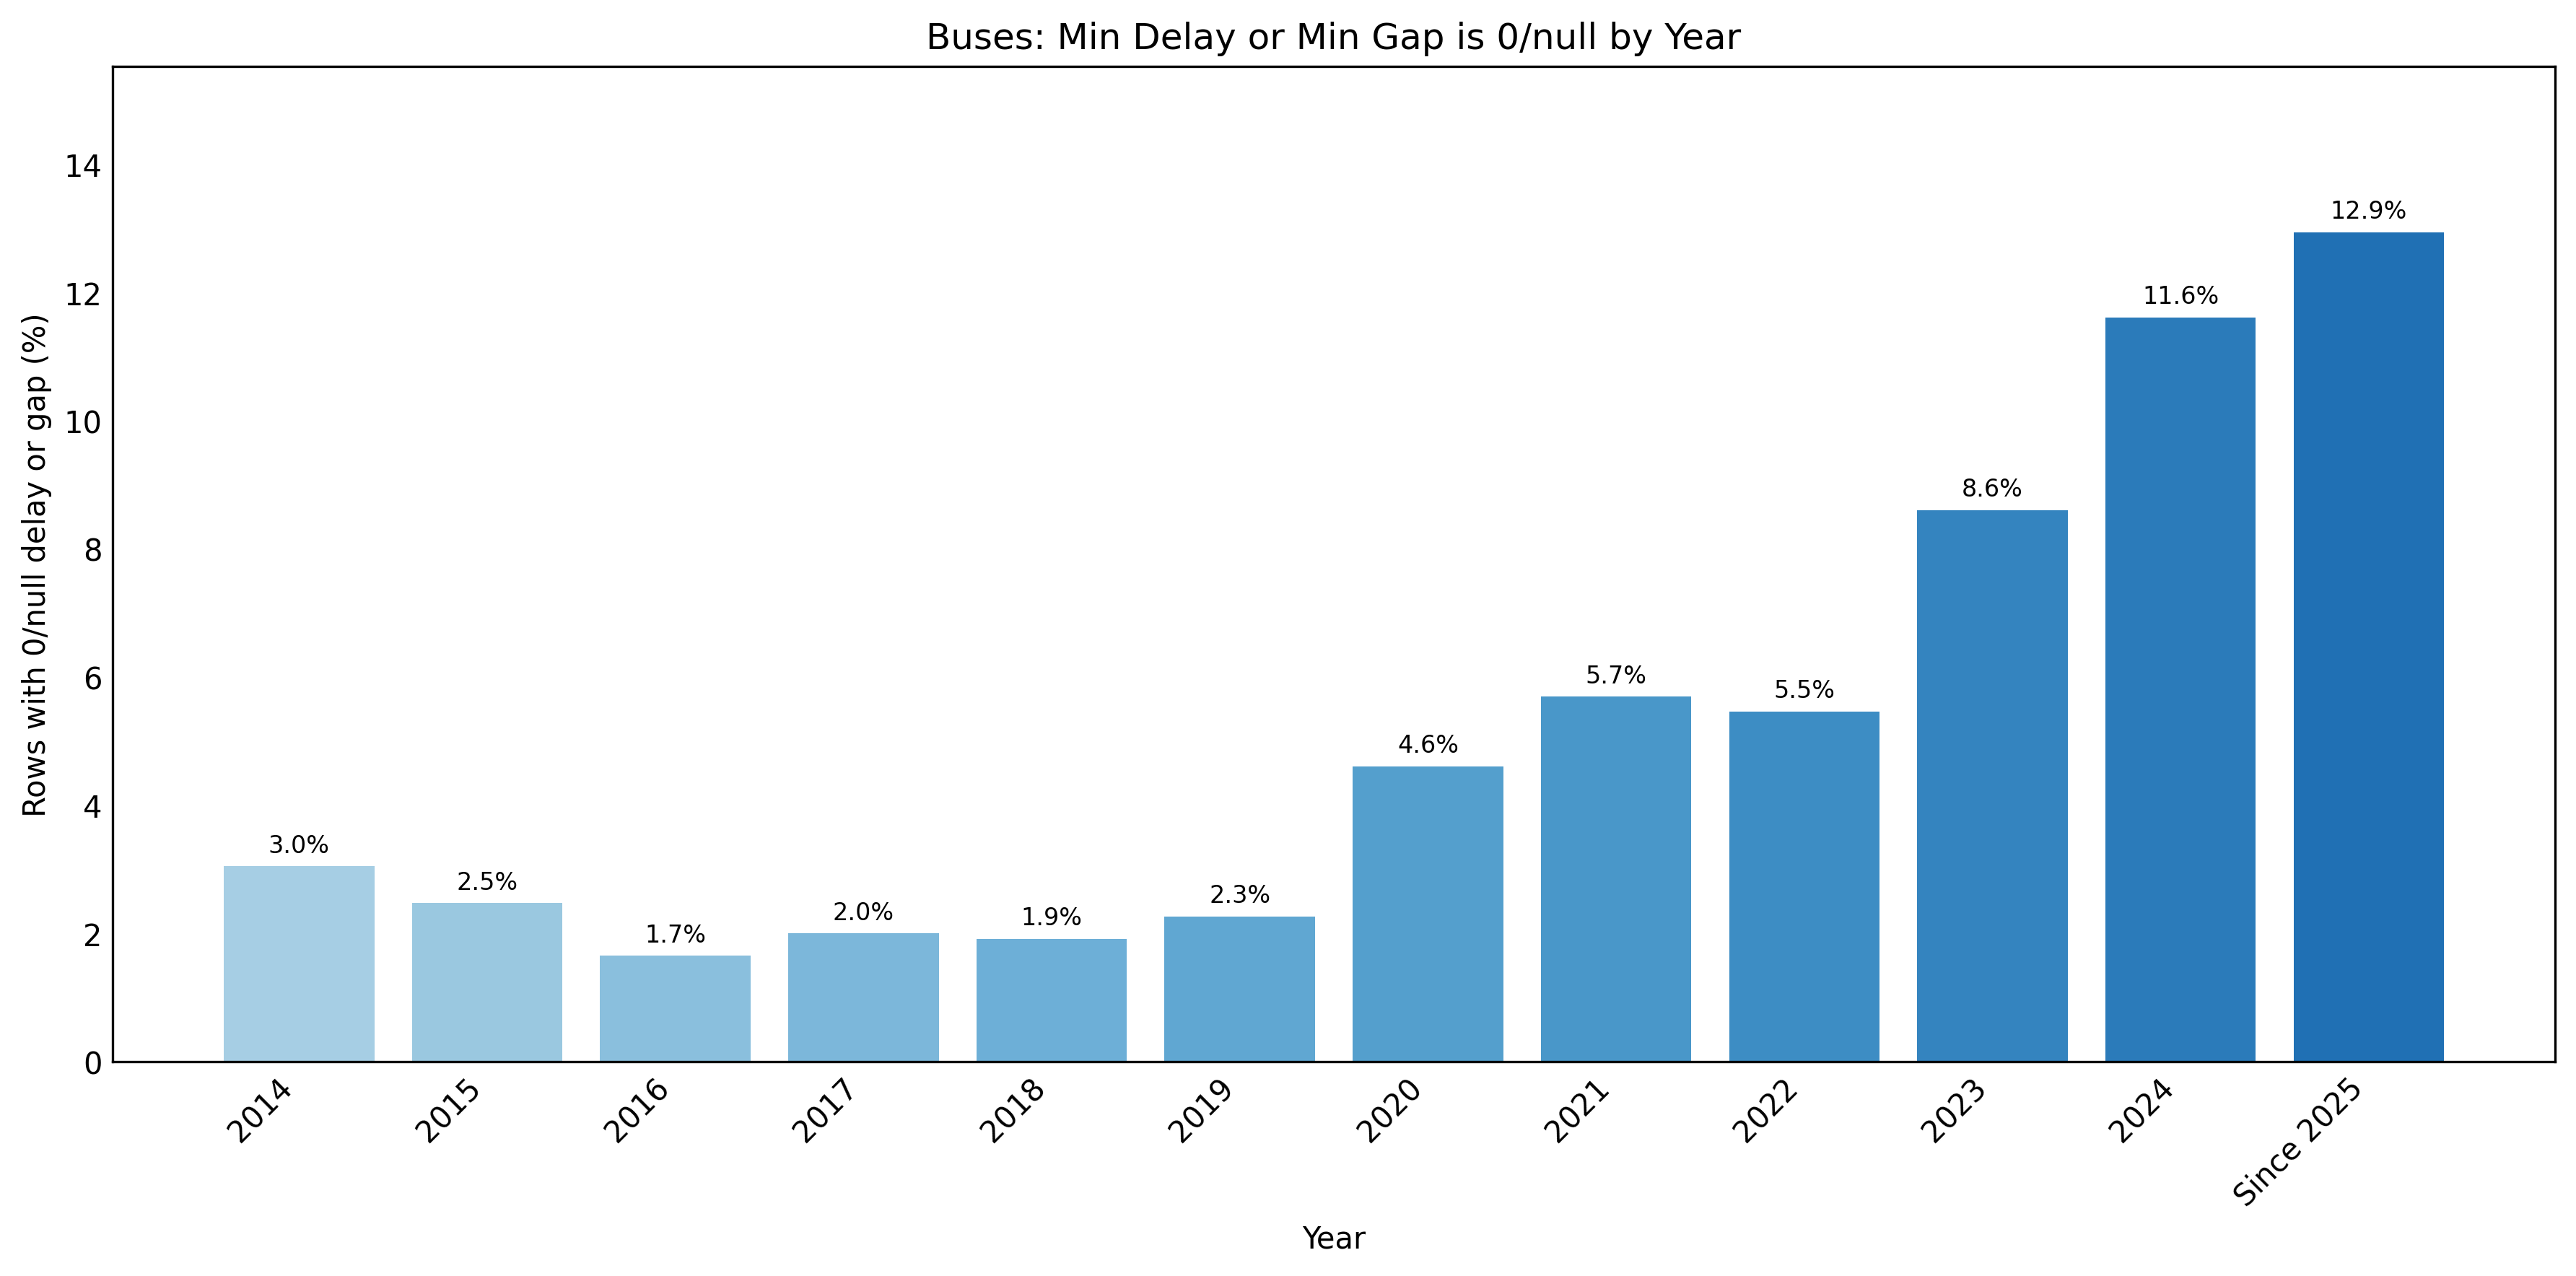
\includegraphics[width=0.9\textwidth]{../data_visualisations/Buses/zero_null_percentage_by_year.png}
    \caption{Buses: percentage of rows with zero or null delay or gap by year.}
    \label{fig:bus-yearly}
\end{figure}

\begin{figure}[htbp]
    \centering
    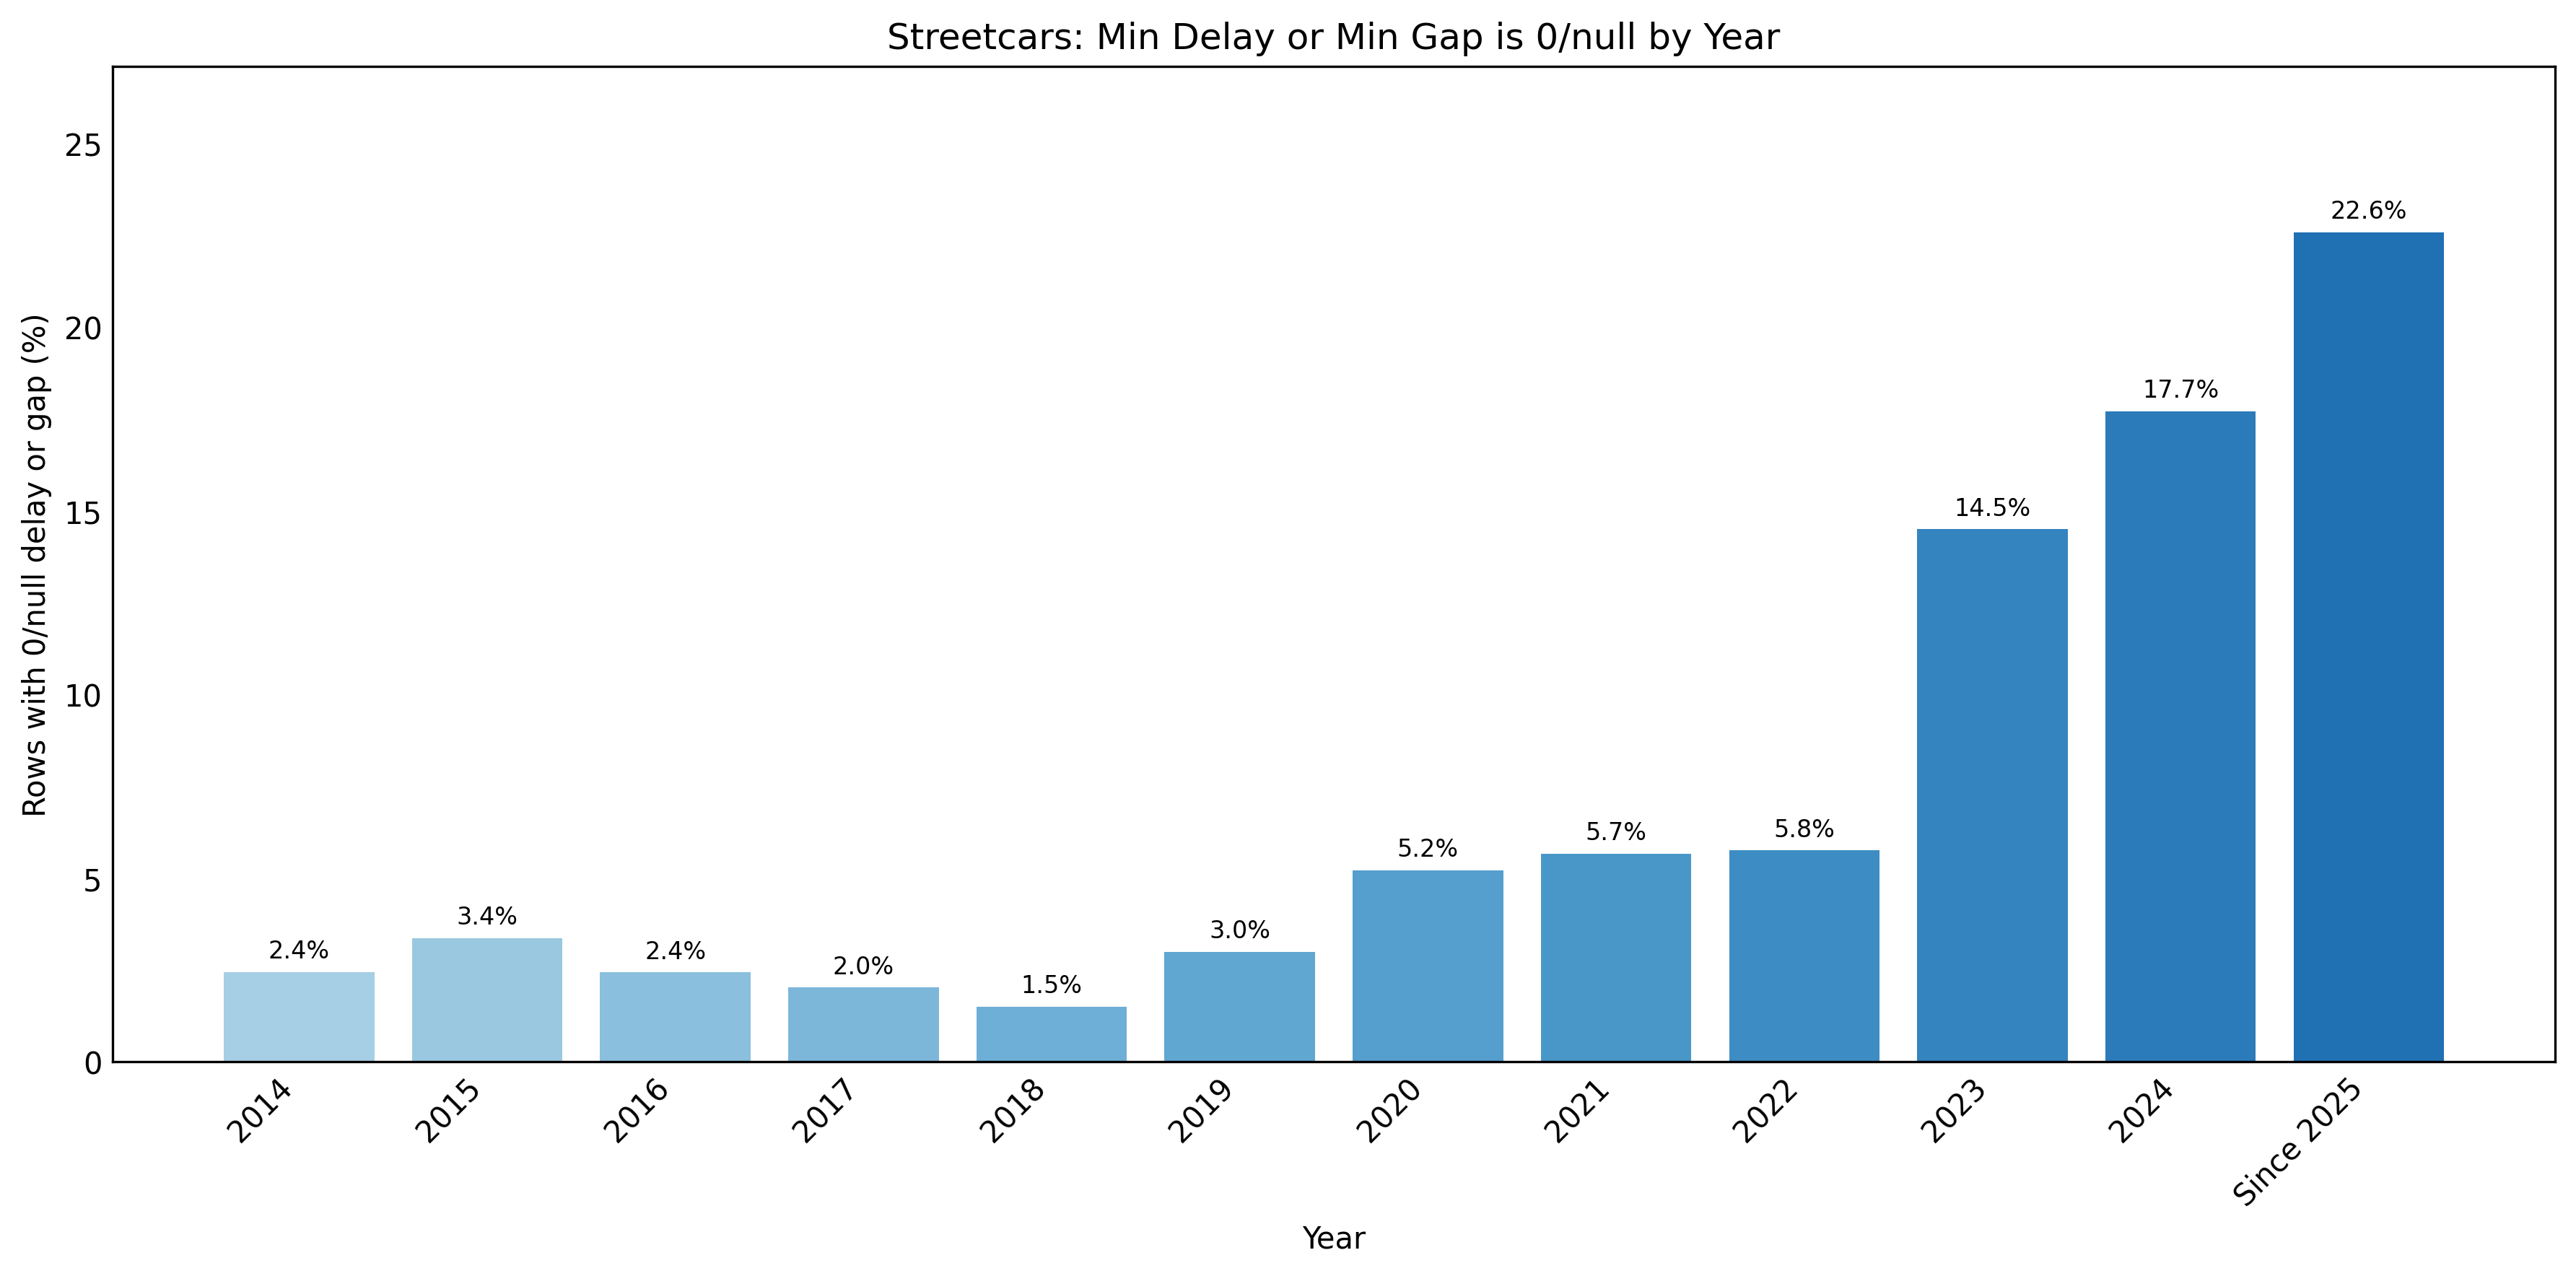
\includegraphics[width=0.9\textwidth]{../data_visualisations/Streetcars/zero_null_percentage_by_year.png}
    \caption{Streetcars: percentage of rows with zero or null delay or gap by year.}
    \label{fig:streetcar-yearly}
\end{figure}

\section{Conclusion}

We consolidated TTC bus and streetcar delay datasets, automated CSV merging, and produced
visualizations that highlight data-quality patterns across years. This work provides a reusable
foundation for further analysis, including geographic mapping and deeper delay trend studies.

\section{Repository Structure}

\begin{table}[htbp]
    \centering
    \begin{tabular}{@{}ll@{}}
        \toprule
        Path & Description \\
        \midrule
        \texttt{raw\_data\_sources/} & Original TTC CSV files \\
        \texttt{scripts/merge\_csv.py} & CSV merge utility \\
        \texttt{scripts/data\_visualiser.py} & Chart generation script \\
        \texttt{data\_visualisations/} & Generated PNG figures \\
        \bottomrule
    \end{tabular}
\end{table}

\end{document}
